\documentclass[tikz, border=10pt]{standalone}
\usepackage{pgfplots}
\pgfplotsset{compat=1.18}
\usepackage{amssymb}

\begin{document}
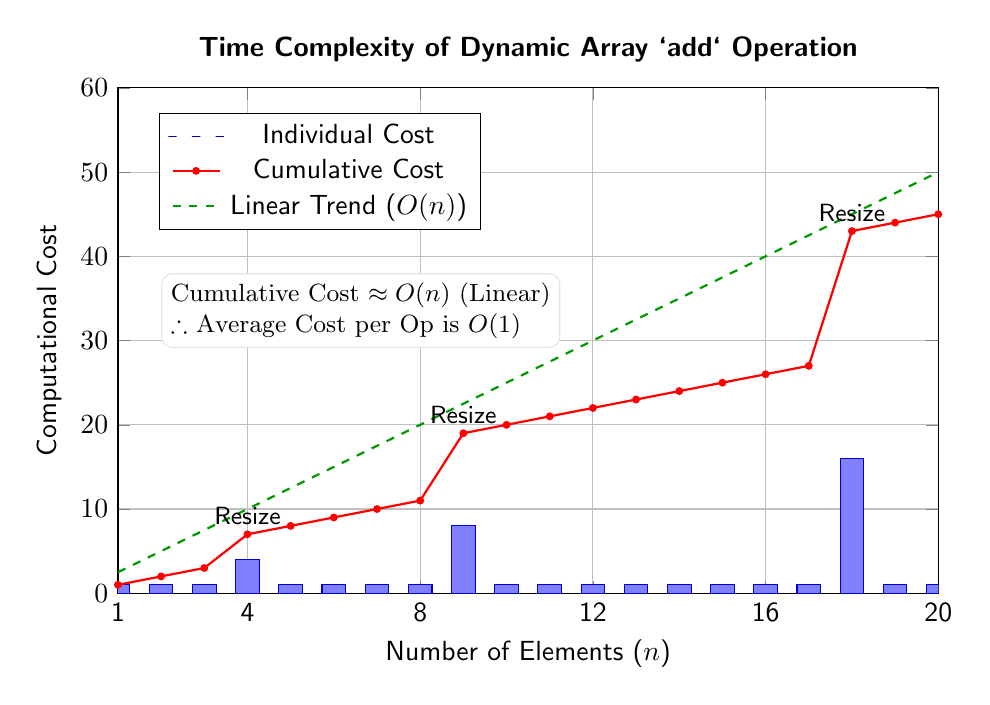
\begin{tikzpicture}[font=\sffamily]
    \begin{axis}[
        title={\textbf{Time Complexity of Dynamic Array `add` Operation}},
        xlabel={Number of Elements ($n$)},
        ylabel={Computational Cost},
        xmin=1, xmax=20,
        ymin=0, ymax=60,
        grid=major,
        width=12cm,
        height=8cm,
        legend style={at={(0.05,0.95)}, anchor=north west},
        xtick={1, 4, 8, 12, 16, 20},
        xticklabels={1, 4, 8, 12, 16, 20},
        ytick={0, 10, 20, 30, 40, 50, 60}
    ]

    % Bar plot for individual operation cost
    % Data from Mermaid: 1, 1, 1, 4, 1, 1, 1, 1, 8, 1, 1, 1, 1, 1, 1, 1, 1, 16, 1, 1
    \addplot[
        ybar,
        fill=blue!50,
        draw=blue!80!black,
        bar width=0.3cm
    ] coordinates {
        (1, 1) (2, 1) (3, 1) (4, 4) 
        (5, 1) (6, 1) (7, 1) (8, 1) (9, 8) 
        (10, 1) (11, 1) (12, 1) (13, 1) (14, 1) (15, 1) (16, 1) (17, 1) 
        (18, 16) (19, 1) (20, 1)
    };
    \addlegendentry{Individual Cost}

    % Line plot for cumulative cost
    % Data from Mermaid line: 1, 2, 3, 7, 8, 9, 10, 11, 19, 20, 21, 22, 23, 24, 25, 26, 27, 43, 44, 45
    \addplot[
        thick,
        color=red,
        mark=*,
        mark size=1pt
    ] coordinates {
        (1, 1) (2, 2) (3, 3) (4, 7) 
        (5, 8) (6, 9) (7, 10) (8, 11) (9, 19) 
        (10, 20) (11, 21) (12, 22) (13, 23) (14, 24) (15, 25) (16, 26) (17, 27) 
        (18, 43) (19, 44) (20, 45)
    };
    \addlegendentry{Cumulative Cost}

    % Trend Line (Linear)
    % Showing that cumulative cost ~= 3n (approximation)
    \addplot[
        thick,
        dashed,
        color=green!60!black,
        domain=1:20,
        samples=2
    ] {2.5*x};
    \addlegendentry{Linear Trend ($O(n)$)}

    % Annotations for spikes
    \node[anchor=south] at (axis cs: 4, 7) {\small Resize};
    \node[anchor=south] at (axis cs: 9, 19) {\small Resize};
    \node[anchor=south] at (axis cs: 18, 43) {\small Resize};

    % Explanation of Linear Trend
    \node[anchor=north west, align=left, fill=white, draw=black!10, rounded corners, font=\small] at (axis cs: 2, 38) {
        Cumulative Cost $\approx O(n)$ (Linear) \\
        $\therefore$ Average Cost per Op is $O(1)$
    };

    \end{axis}
\end{tikzpicture}
\end{document}
